\title{Partitioned Matrices and Matrix Multiplication}
\subtitle{\SubTitleName}
\institute[]{\Course}
\author{\Instructor}
\maketitle  







\frame{\frametitle{Topics and Objectives}
\Emph{Topics} \\
\TopicStatement
\begin{itemize}
    \item partitioned matrices (or block matrices)
    \item matrix multiplication with partitioned matrices
\end{itemize}

\vspace{0.5cm}

\Emph{Objectives}\\

\LearningObjectiveStatement

\begin{itemize}
    \item apply partitioned matrices to solve problems regarding matrix multiplication 
\end{itemize}

\vspace{0.25cm} 

%\Emph{Motivating Question} \\
%You have three group of variables $ X_1$, $ X_2, $ and $ X_3$. Within each group, they have many relationships, but between groups, only a few. What would the resulting matrix of relationships look like? 

}


\frame{\frametitle{Multiple Perspectives}


{\small \textit{``Mathematics is not about numbers, equations, computations, or algorithms. Mathematics is about understanding." } \\ - William Paul Thurston \\}

\vspace{12pt}

\pause

Multiple perspectives of the same concept is a theme of this course; each perspective deepens our understanding. In this section we explore another way of representing matrices and their algebra that gives us another way of thinking about them. 

}



\frame{\frametitle{What is a Partitioned Matrix?}

% \Emph{Example} \\
This matrix: 
$$A = \begin{pmatrix} 3&1&4&1&0\\1&6&1&0&1\\0&0&0&4&2\end{pmatrix}$$

\pause 

can also be written as:

\begin{equation*}
A = 
\begin{pmatrix}
\begin{pmatrix}
3 & 1 & 4 \\ 1 & 6 & 1
\end{pmatrix}  
& 
\begin{pmatrix}
1 & 0 \\ 0 & 1 
\end{pmatrix}
\\[12pt] 
\begin{pmatrix}
0 & 0 & 0 
\end{pmatrix}
& 
\begin{pmatrix}
4 & 2
\end{pmatrix}
\end{pmatrix}
= 
\begin{pmatrix}
A _{1,1} & A _{1,2} \\ A _{2,1} & A _{2,2} 
\end{pmatrix}
\end{equation*}
We partitioned our matrix into four \Emph{blocks}, each of which has different dimensions.

}

\frame{\frametitle{Why are Partitioned Matrices Useful?}


    Partitioned matrices can give a succinct representation of a matrix. 
    
    \begin{equation*}
    \begin{pmatrix}
    1 & 0 & 0 & \ast & \cdots & \ast 
    \\
    0 & 1 & 0  & \ast & \cdots & \ast 
    \\
    0 & 0 & 1 & \ast & \cdots & \ast 
    \\
     0 & 0 &  0 &  0 & \cdots & 0
     \\
      0 & 0 &  0 & 0 &  \cdots & 0
    \end{pmatrix}
    =
    \begin{pmatrix}
    I_3 & F \\ 0 & 0 
    \end{pmatrix}
    \end{equation*}
    
    \pause 
    
    This can be useful when studying something called the \Emph{null space} of $A$, which we will define later in this course.

}






\frame{\frametitle{Recall: the Row Column Method}

Recall the \Emph{row column} method for matrix multiplication. 

\pause 
\begin{center}\begin{tikzpicture} \node [mybox](box){\begin{minipage}{0.95\textwidth}

Let $ A$ be $ m \times n$ and $ B$ be $ n \times p$ matrix. Then, the $ (i,j)$ entry of $ AB$ is 
\begin{equation*}
\operatorname {row}_i A  \cdot   \operatorname {col}_j B . 
\end{equation*}
This is the \Emph{Row Column Method} for matrix multiplication.

\end{minipage}};
\node[fancytitle, right=10pt] at (box.north west) {Theorem};
\end{tikzpicture}\end{center}

\pause 
\Emph{Example}$$
AB = \spalignmat{1 0 1;0 1 1} \spalignmat{2 -1;0 -1;0 1}= 
$$



}





\frame{\frametitle{The Row Column Method for Block Matrices}

    Partitioned matrices can be multiplied using this method, as if each block were a scalar (\textit{provided each block has appropriate dimensions so that products are defined}).
    
    \vspace{12pt}
    
    \pause
    
    \Emph{Example}\\
    Compute the matrix product using the given partitioning. 
    $$
    AB = \spalignmat{1 0 1;0 1 1} \spalignmat{2 -1;0 -1;0 1}= 
    \spalignmat{I_2 X}\spalignmat{U ; Y}
    $$
    Where $X = \spalignmat{1;1}, U = \spalignmat{2 -1;0 1}, Y = \spalignmat{0 1}$.
}








% \frame{\frametitle{Using the Row Column Method to Construct an Inverse}

% Recall, using our formula for a $2\times 2$ matrix,  $ \begin{pmatrix}
% a & b \\ 0 & c 
% \end{pmatrix} ^{-1} = \frac 1 {ac} \begin{pmatrix}
% c &  -b \\ 0 & a 
% \end{pmatrix}$.

% \vspace{0.5cm} 

%     \Emph{Example}: Suppose $ A \in \R^{ n \times n}$, $B \in \R^{n\times n}$, and $C \in \R^{n\times n}$ are invertible matrices. Construct the inverse of $
%     \begin{pmatrix}
%         A & B \\ 0 & C 
%     \end{pmatrix}
%     $.

% } 


\frame{\frametitle{Summary}

    \SummaryLine \vspace{4pt}
    \begin{itemize}\setlength{\itemsep}{8pt}
        \item using partitioned matrices to solve problems regarding matrix multiplication  
    \end{itemize}
    \vspace{4pt}
    Although not part of our course, matrix partitioning is often used to help derive new algorithms because they give a more concise representation of a matrix and of operations on matrices. 
}






% COLUMN ROW METHOD USUALLY NOT NEEDED IN THIS CLASS
% \frame{\frametitle{The Column Row Method (if time permits)}

% A column vector times a row vector is a matrix. For example,

% $$
% \begin{pmatrix}
% 1 \\ 0 \\ 2
% \end{pmatrix} 
% \begin{pmatrix}
% 1 & 3  
% \end{pmatrix} 
% = 
% %\begin{pmatrix} 1 & 3 \\ 0 & 0 \\ 2 & 6 \end{pmatrix}
% $$

% \begin{center}\begin{tikzpicture} \node [mybox](box){\begin{minipage}{0.8\textwidth}

% Let $ A$ be $ m \times n$ and $ B$ be $ n \times p$ matrix. Then,  
% \begin{align*}
%  AB &= 
%  \begin{pmatrix}
% \operatorname {col}_1 A & \cdots & \operatorname {col}_n A 
% \end{pmatrix}
%  \begin{pmatrix}
% \operatorname {row}_1 B \\ \vdots \\  \operatorname {row}_n B 
% \end{pmatrix}
% \\&= 
% \underbrace{
% \operatorname {col}_1 A \operatorname {row}_1 B + \cdots \operatorname {col}_n A \operatorname {row}_n B } 
% _{\textup{$ m \times p$ matrices}} 
% \end{align*}
% This is the \Emph{Column Row Method} for matrix multiplication.

% \end{minipage}};
% \node[fancytitle, right=10pt] at (box.north west) {Theorem};
% \end{tikzpicture}\end{center}


% }

% %% FRAME
% \begin{frame}\frametitle{The Strassen Algorithm: An impressive use of partitioned matrices}

% Naive Multiplication of two $ n \times n$ matrices $ A$ and $ B$ requires $ n ^3 $ arithmetic steps. 
% Strassen's algorithm \Emph{partitions} the matrices, makes a very clever sequence of multiplications, additions, to reduce the computation to $ n ^{2.803\ldots }$ steps.  


% \begin{center}
%     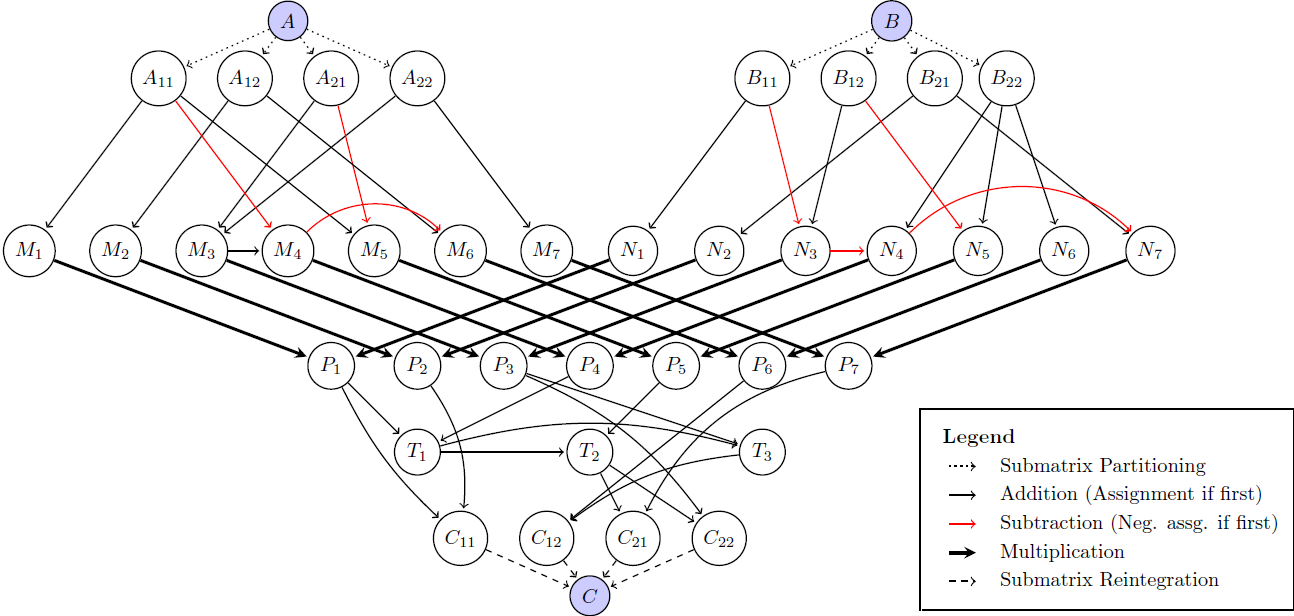
\includegraphics[width=0.85\textwidth]{Chapter2/images/StrassenAlgorithm} 
% \end{center}

% \center{\small{{\color{Grey}{\small\textit{Students aren't expected to be familiar with this material. It's presented to motivate matrix partitioning.}}}}}

% \end{frame}


% \begin{frame}\frametitle{The Fast Fourier Transform (FFT)}

% The FFT is an essential algorithm of modern technology that uses partitioned matrices recursively. 

% \begin{equation*}
% G_0 =  
% \begin{pmatrix}
% 1 
% \end{pmatrix}, \qquad  G _{n+1} = 
% \begin{pmatrix}
% G _n  & - G_n \\ G_n & G_n 
% \end{pmatrix}
% \end{equation*}

% \bigskip 

% \begin{columns}
% \begin{column}{.5\textwidth}
% \begin{center}
%  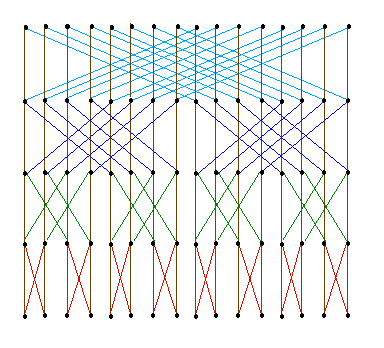
\includegraphics[width=0.8\textwidth]{Chapter2/images/fft1} 
% \end{center}
% \end{column}
% \begin{column}{.5\textwidth}
% \vskip .75cm
% The recursive structure of the matrix means that it can be computed in nearly \Emph{linear} time. This is an incredible saving over the general complexity of $ n ^{3}$.  It means that we can compute $ G_n x$, and $ G ^{-1}_n$ very quickly.  
% \end{column}
% \end{columns}


% \center{\small{{\color{Grey}{\small\textit{Students aren't expected to be familiar with this material. It is presented to motivate matrix partitioning.}}}}}

% \end{frame}